\documentclass{template/socthesis}

\usepackage{subcaption}
\usepackage{amsmath}
\usepackage{enumitem}
\usepackage{hyperref} % balíček pro hypertextové odkazy

\usepackage{color} % balíček pro obarvování textů
% \color{blue}
\usepackage{xcolor}  % zapne možnost používání barev, mj. pro \definecolor
\definecolor{mygreen}{RGB}{0,150,0} % nastavení barev odkazů 
\definecolor{myblue}{RGB}{0,0,200} 
\definecolor{commentgreen}{RGB}{0,100,0} % nastavení barev pro příklady z C++
\definecolor{deepblue}{rgb}{0,0,0.7}
\definecolor{deepred}{rgb}{0.6,0,0}
\definecolor{deepgreen}{rgb}{0,0.5,0}

\hypersetup{colorlinks=true, linkcolor=myblue, urlcolor=mygreen, citecolor=blue, anchorcolor = magenta,
	linktocpage = true, frenchlinks } % nastavení barvy odkazů 

\addbibresource{text.bib}

\titlecz{Postav si svého prvního robota}
\titleen{Build your first robot}
\author{Tomáš Vavrinec}
\field{10}
\school{Střední průmyslová škola a Vyšší odborná škola Brno, Sokolská}
\mentor{Mgr.Miroslav Burda}
\mentorstatement{Mgr.Miroslava Burdy}

% Změňte, pokud se liší
%\region{Jihomoravský}
%\placefooter{Brno 2017}



\begin{document}

\maketitle

\makecopyrightstatement{V~Brně}

\makethanks{Děkuji svému školiteli Mgr. Miroslavu Burdovi za obětavou pomoc, podnětné připomínky a nekonečnou trpělivost, kterou mi během práce poskytoval.}

\pagestyle{empty}

\section*{Anotace}

Cílem práce je  vyvinout vhodnou levnou a rozšiřitelnou vzdělávací pomůcku -- řídící desku, která umožňuje názorně předvést vlastnosti senzorů a pohonů a která bude schopná řídit například i amatérské soutěžní roboty nebo školní ukázku výrobní linky. Dále vyvinout snadno dostupného robota, kterého tato řídící deska bude řídit.

Tato práce se zabývá návrhem a výrobou řídící desky Schoolboard a robota Schoolbot a jejich použitím při výuce dětí v zájmovém vzdělávání a při školní výuce předmětů elektroniky, automatizace, programování a dalších. 

\subsection*{Klíčová slova}
robot; vyuka robotiky; řídící deska; ESP32

\vspace{20mm}

\section*{Annotation}
%todo 

\subsection*{Keywords}

\newpage
\pagestyle{plain}

\tableofcontents % vysází obsah

%%% Začátek práce
\setcounter{figure}{0}
\setcounter{table}{0}
\newpage

\chapter*{Úvod}
\addcontentsline{toc}{chapter}{Úvod} % přidá položku úvod do obsahu
Moje práce má za cíl vytvořit pomůcku (robota) pro praktické seznámení s~elektonikou, robotikou a programováním pro:  

\begin{itemize}
	\item účastníky volnočasových kroužků robotiky, elektroniky a podobných
	\item studenty středních škol, především oborů elektronika, automatizace, robotika, ale i pro předměty informatika nebo fyzika
	\item další začínající zájemce o elektoniku a robotiku. 
\end{itemize}


 Pokud zájemce -- začátečník  o elektroniku a nebo hobby robotiku absolvuje \uv{blikání ledkou}, obvykle chce pokračovat stavbou svého prvního robota (podle hesla: \uv{Ať se to hýbe!}). Když se 
 rozhlédne kudy dál, zjistí, že všechny dostupné možnosti jsou tak či onak dost problematické (viz kapitola \ref{konkurence}). 
 
 Podobná situace nastává ve škole, kdy například funkci probíraných senzorů, enkodérů a podobně někdy není na čem prakticky ukázat. To se týká především situace, kdy učitel chce, aby studenti s robotem sami pracovali, například ve dvojicích.   

Řídící deska \textbf{Schoolboard} a robot \textbf{SchoolBot} jsou primárně navrženy pro volnočasový vzdělávací kroužek robotiky pořádaný na naší škole a jsou určeny pro začátečníky. Jako takoví dávají účastníkům kroužku možnosti, které má prakticky každý soutěžní robot, konkrétně pohon pro pohyb na hřišti, klepeta pro manipulaci s herními prvky a senzory pro samostatnou orientaci na hřišti. 
\newpage

 Takový robot by měl mít: 

\begin{itemize}
	\item \textbf{modulární senzoriku} -- být schopný připojit na sebe různé senzory 
	
	\item \textbf{rozšiřitelnou konstrukci} -- možnost i velké úpravy, změn a rozšíření konstrukce robota, připojení různých pohonů (motory, serva)
	
	\item \textbf{bezdrátové řízení}
	
	\item dostatečně \textbf{tuhou konstrukci}
	
	\item  \textbf{možnost programovat v C++}, které je dnes standardem v této oblasti
	
	\item a hlavně: \underline{\textbf{nízkou pořizovací cenu}}, protože bez ní jsou všechny ostatní příznivé vlastnosti bohužel téměř na nic 
	
\end{itemize}

Ideálně by si takového robota učastníci kroužku měli být schopni postavit, spájet a oživit (podle pokynů vedoucího) sami. 

%\section{SchoolBot}


%\section{BlackBox}
%BlackBox je elektronicky ovládaný trezor, který je s vhodnou úpravou schopen i jezdit na vlastních kolech. Pro začátečníky má i čistě mechanickou variantu bez elektroniky, ta však muže sloužit jen jako trezor a nemá ostatní možnosti které má až elektronická varianta. Elektronická varianta má rozmanité senzory, díky kterým muže nabývat různých podob od trezor po hodiny.


\newpage

\chapter{Proč vytvářet vlastní roboty?}

Proč vlastně vytvářet vlastní elektroniku i mechaniku, když je na trhu tolik různých robotu a vozítek? Konkurenční roboti, kteří se běžně prodávají, jsou totiž většinou velmi drazí a často nemají ani moc možností. Například známé LEGO Mindstorms, u kterého se cena základní sady pohybuje nad sedmi tisíci korunami [], %todo
 je vzhledem ke svým možnostem ohromně předražené.
 
Při vytváření pokročilejších aplikací potřebuje tvůrce znalost technických specifikací robota a jeho vnitřního fungování. U většiny komerčních robotů však není kompletní technická dokumentace volně dostupná.


\section{Konkurence} \label{konkurence}

\subsection{LEGO Mindstorms EV3}

LEGO Mindstorms je známé svou jednoduchostí. Základní roboti se s touto sadou dají sestavit velmi rychle, což poskytuje hlavně začátečníkům motivaci, neboť již s poměrně malým úsilím sestaví něco, co na první pohled funguje. Dílky LEGa však nejsou moc pevné a konstrukce z nich postavená jich tedy vyžaduje velké množství, aby byla obstojně tuhá. To se samozřejmě dá vyřešit tím, že si člověk udělá konstrukci z jiného materiálu, potom ale odpadá výhoda jednoduchosti stavby.

Možnosti robota se z velké části odvíjí od senzoriky. LEGO trpí na nedostatek senzorů. Nejen, že v základní sadě je, krom tlačítka, od každého sensoru jen jeden kus. Ale ani kostka, řídící centrum LEGa, nedokáže číst víc než čtyři senzory naráz. Je pravda že LEGO má možnost spojovat několik kostek dohromady, to však samozřejmě vyžaduje mít jich víc, což je při ceně LEGa poměrně drahé.


LEGO má své vlastní programovací prostředí, které je většinou pro začátečníky dobré. Jakmile však uživatel chce vytvářet vetší program, prostředí velmi rychle ztratí užitečnost. Vetší programy jsou v grafickém prostředí velmi nepřehledné. Navíc prostředí LEGa může být u větších programů nestabilní. Existují však i prostředí, ze kterých se dá lego programovat textově, například v jazyku C++, což je u složitějších programu přehlednější a také méně náročné pro počítač.

\subsection{Mbot}
Mbot je oproti legu daleko levnější (cena se pohybuje kolem osmnácti set korun za kus) ale trpí stejným, nebo i větším, nedostatkem sensorů. 

Co se konstrukce týče, problémy s pevností u Mbota není, ale zase se nedá snadno upravit. Konstrukce je totiž hliníková, což je v pořádku, pokud není potřeba konstrukci výrazně upravovat. Robota je ale většinou třeba přizpůsobit konkrétnímu užití.
 Ze zkušenosti se nejvíce osvědčilo dřevo, které se dá jednoduše upravovat bez větší námahy a zároveň není problém z něj udělat dostatečně tuhou konstrukci. Hliník se však tak lehce ručně upravovat nedá.
 
Mbot je založen na procesoru ATmega328, což je stejný procesor, jaký se používá i u velice známého Arduina. %todo odkazy
To znamená, že některé programy, které jsou napsané pro Arduino, je možné spustit i zde.

\subsection{Edison V2.0}
Edison %todo odkaz podobně i dál
je velmi podobný LEGu a má i podobné problémy. Opět nedisponuje velkým počtem senzorů, ale oproti LEGu je alespoň daleko levnější. 

Stejně jako LEGO má i Edison vlastní grafické programovací prostředí, bohužel jsem jej nikdy nepoužíval, ale vypadá velmi podobně jako prostředí LEGa. Myslím si proto, že stejně jako prostředí LEGa bude i toto velice dobré na malé prográmky pro děti, ale nevhodné pro obsáhlé programy.

Všechny senzory má Edison uvnitř sebe a nedají se proto dovést na místo, kde je uživatel nejvíc potřebuje. Uživatel se proto musí přizpůsobit rozložení senzorů na řídící jednotce, stejně tak se nedá vyvést ani nic jiného. Jediné, co se dá, je vyměňovat kola (například za nějaké ozubení) a pomocí toho si pak dovést náhon z motoru na potřebné místo.


\subsection{Mbot}
Mbot je oproti legu daleko levnější (cena se pohybuje kolem osmnácti set korun za kus) ale trpí stejným, nebo i větším, nedostatkem sensoru. Co se konstrukce týče, problémy s pevností u Mbota není ale zase se nedá snadno upravit. Konstrukce je totiž hliníková, což je v pořádku, pokud není potřeba konstrukci výrazně upravovat. Robota je ale většinou třeba přizpůsobit konkrétnímu užití, ze zkušenosti se nejvíce osvědčilo dřevo, které se dá jednoduše upravovat bez větší námahy a zároveň není problém z něj udělat dostatečně tuhou konstrukci. Hliník se však tak lehce ručně upravovat nedá. Mbot je založen na procesoru ATmega328 což je stejný procesor jaký se používá i u velice známého arduina. To znamená že některé programy, které jsou napsané pro arduino je možné spustit i zde.

\subsection{Edison V2.0}
Edison je velmi podobný legu a mí i podobné problémy. Opět nedisponuje velkým počtem senzoru ale oproti legu je daleko levnější. Stejně jako lego má i Edison vlastní grafické programovací prostředí, bohužel jsem jej nikdy nepoužíval, ale vypadá velmi podobně jako prostředí lega. Myslím si proto, že stejně jako prostředí lega bude i toto velice dobré na malé prográmky pro děti, ale nevhodné pro obsáhlé programy. Všechny senzory má Edison uvnitř sebe a nedají se proto dovést na místo kde je uživatel nejvíc potřebuje. Uživatel se proto musí přizpůsobit rozložení senzoru na řídící jednotce, stejně tak se nedá vyvést ani nic jiného. Jediné, co se dá, je vyměňovat kola (například za nějaké ozubení) a pomocí toho si pak dovést náhon z motoru na potřebné místo.


\subsection{OZOBOT}
Ozobot je mini robot, z toho vyplývají jeho největší výhody i nevýhody. Například pochopitelně není dělaný na to, aby cokoli vozil nebo jakkoliv stěhoval. Téměř se nedá upravovat, na to ale opět není dělaný. Jeho účel je především jezdit po čáře a vykonávat příkazy na ní zapsané pomocí barevných vzorů. Přes to že se novější verze dají i programovat, jejich funkce jsou pořád mířené do velké míry právě na čáru a barevné příkazy na ní.

\subsection{Asuro}
Asuro je robot postavený kolem základní desky. Jedná se o stavebnici, ale přesto nemá ani jednoduché pomůcky pro možnost přesné stavby. Asuro má mezi koly a motorem převodovku, která se ukládá do jakýchsi ložisek. Ta se bez jakéhokoli zapozicování napájí na plochu desky. Výsledkem je téměř nemožnost uložit kola převodovky přesně.


\subsection{Microbit}
Microbit je především řídící deska se senzory a výstupními ledkami. Není to primárně vozítko, přestože existují konstrukce, které jsou určené právě pro řízení microbitem. Taková konstrukce však muže využívat pouze serva, nebo musí mít vlastní řízení motoru. Microbit totiž motory řídit nedokáže sám, dokáže řídit jen serva, která si řízení řeší sama. Toto však není velký problém, protože existuje více různých konstrukcí, které právě toto řeší. 

Microbit má překvapivě docela dost senzorů přímo na základní destičce. Podle mých informací kompas, který je přímo na desce téměř nefunguje, ale vzhledem k tomu, co všechno na sobě malá destička Microbit má, to není až taková tragédie. Kompas je stejně často potřebné dostat co nejdál od zbytku robota, kvůli všemožnému rušení, takže by se i tak dost možná používal jako externí součástka.

Microbit má zároveň matici ledek, na které si uživatel muže zobrazova,t co se mu zlíbí a zároveň se jimi dá i měřit světelnost okolí. Používání led diod jako fotodiod sice není tak přesné, nicméně to jde a je to zajímavé řešení.

%todo nevýhody microbitu? 

\subsection{Shrnutí}
Komerční systémy jsou většinou velmi drahé, mívají nedostatek senzorů, mívají měkkou nebo obtížně upravitelnou konstrukci a také nemají moc velký výkon ani přesnost pohonu.

Možná si říkáte, proč mi záleží na tom aby robot pro začátečníky měl všechny tyto možnosti. Vždyť člověku, co nikdy robota nestavěl, by to mohlo být skoro jedno. Ano, ale já chci, aby se na prvním robotu, které si zájemce postaví, dalo stavět dál. Aby bylo vidět, že si z robota, který toho moc neuměl, může uživatel postavit něco, co by třeba mohlo jezdit na soutěže a vyhrávat. % ahoj ahoj 

\begin{table}[h]
	\centering
	\begin{tabular}{|l|l|l|l|l|l|l|}
		\hline
		\textbf{robot }			& modulární   & rozšiři- & bezdrátové  & tuhá  & nízká & C++\footnote{Možnost naprogramování robota v C++.} \\
		 & senzorika & telnost & řízení & konstrukce & cena &  \\
		 \hline
		Mbot 			& 0 				& 0 			& 0 			& 1 			& 0			& 0	\\ 
		LEGO\footnote{myšleno LEGO MINDSTORMS} 	& 1/2 				& 1 			& 1 			& 0 			& 0			& 1/2	\\ 
		Edison 			& 0 				& 0 			& 1/2 			& 1/2 			& 1			& 0	\\ 
		OZOBOT			& 0					& 0				& 1 			& 1				& 0			& 0	\\
		Asuro			& 0					& 0				& 0 			& 0				& 0			& 1	\\
		Microbit		& 0					& 1				& 1 			& 1				& 0			& 0	\\
			\textbf{SchoolBot} 		& \textbf{1} 				& \textbf{1} 			& \textbf{1} 			& \textbf{1} 			& \textbf{1} 		& \textbf{1}	\\ 
		\hline
	\end{tabular}
	\caption{Srovnání možností dostupných komerčních systémů pro hobby roboty}
\end{table}

\chapter{SchoolBot}

\section{Z čeho se SchoolBot skládá?}
SchoolBot je komplet, skládající se ze řady jednotlivých dílků, které nebudu popisovat samostatně pro začátek systém rozdělím na elektroniky a mechaniku.

\subsection{Elektronika}

Elektronika je především řídící deska SchoolBoard kterou shrnuji v samostatné kapitole a detailně rozebírám v přílohách. Krom desky obsahuje SchoolBot battery pack, motory s enkodéry a inteligentní serva LX15D[viz zdroje] které uvádí do provozu klepeta, nástroj pro možnost manipulace s objekty při soutěžích především herními prvky.

\subsubsection{battery pack}

Battery pack je sestaven ze dvou li-on baterii 18650 které jsou pomocí DPS spojeny v jeden celek. Připojení do robota je pak zajištováno pomocí dutinek a to každý článek zvlášť, serializují se až po vložení do robota. Důvodem pro vyvádění obou článku zvlášť je nabíjení, to je totiž realizováno pomocí lineárních nabíjecích modulu, které se napájejí z USB a každý článek se nabíjí zvlášť.
Aby se battery pack nedal omylem připojit s opačnou polaritou je vyřešen tak že se dá při připojení otočit dvěma způsoby a oba mají správnou polaritu, dokonce i stejné pořadí článků.

\subsubsection{motory s enkodéry}

SchoolBot používá levné motory s plastovou převodovkou které v základu enkodéry nemají. Enkodéry si proto SchoolBot řeší sám, a to pomocí magnetu a dvou halových sond. Takto vyrobený inkrementální enkodér pak vyhodnocuje procesor na řídící desce.

\subsection{Mechanika}

Mechanika SchoolBota je celá z překližky vypálené pomocí laserového řezáku. Je stavěná kruhově aby se robot nemohl zaseknout v nějakém rohu a v přední části má umístěná klepeta kterými je schopna nabírat a převážet různé objekty. 

\subsubsection{Uložení kol a motoru}

Kola nejsou jen tak nasazená na motor. Aby se nevyvracela, a tím pádem méně zatěžovala převodovku motoru, jsou z druhé strany podepřena a uchycena k obvodu konstrukce.
Celí motor i s kolem je pak z části držen podporou kola ale především je celí motor vložen do těsné šachty kde se nemůže otočit ani posunout jiným směrem než vzhůru a následně je přitlačen palubou která se přišroubuje čtyřmi šrouby. Takovéto řešení umožnuje jednoduchý přístup k motoru.


\chapter{SchoolBoard}

\section{Popis desky}

Deska má k dispozici

\begin{itemize}
	\item třicetidvoubitový procesor ESP32 s taktovací frekvencí 240~MHz a napájecím napětím 3,3 V 
	\item flash pamětí 4 MB (dělají se i verze s 8 a 16 MB), 520 KB SRAM, WI-Fi, Bluetooth, 28 vstupně výstupních piny, dva ADC převodníky (jeden s 6 piny a druhý s 10 piny), jedním DAC převodníkem s dvěma piny, tři UARTy, dvě SPI, tři I2C(jedno je použito interně pro flash) atd.
	
	\item Motorový driver DRV8833, který umožnuje řídit dva stejnosměrné motory nebo jeden krokový motor.
	
	\item Tři konektory na inteligentní serva LX-15D nebo LX-16A. Deska dokáže řídit až 254 těchto serv. Serva se totiž dokáží řetězit za sebe, ale pokud potřebují větší proud (když podávají větší kroutící moment), ubytek napětí na kabelech je už moc velký, aby serva mohla využít plný výkon. Proto jsou na desce konektory tři a ne jen jeden.
	
	\item Čtyři uživatelská tlačítka.
	
	\item Tři uživatelské LED a jedna LED signalizující zapnutý stav.
	
	\item Možnost měření napětí baterie.
	
	\item Hardwarové řešení startu a vypínání (dá se použít i jako nouzový vypínač). Tlačítka na zapínání a vypínání jsou jak přímo na desce, tak jsou i vyvedena na pinheady pro možnost připojení externího řízení.
	
	\item Konektor na připojení motorů s enkodérem.
	
	\item Deska operuje na napětí 3,3~V, ale aby byla schopná komunikovat i s periferiemi operujícími
	na napětí 5~V, jsou čtyři piny opatřené převodníkem napěťových úrovní.
	Piny IO35, IO32, IO14 a IO12 jsou tedy schopny operovat jak na napětí 3,3~V, tak na 5~V.
	
	Piny jsou teoreticky schopné pracovat i na napětí vyšším, záleží na součástce IM3
	(step-down nebo stabilizátor 7805), která napájí převodník. Pokud bude IM3 dodávat jiné napětí, bude toto napětí i na 5~V pinech (napětí nesmí klesnout pod 4,5~V jinak procesor nedostane dost proudu).
	
	\item Vyvedení 5~V napájení je na oddělené stabilizaci (součástka IM4) pro možnost napájení jiným napětím.
	
	\item Deska má také vyvedeny všechny piny ESP32, které nejsou spojeny 
	s hlavní funkcí desky (řízení motorů) a není problematické se o ně starat při bootu ESP32.
	
	\end{itemize}
\subsection{Možné periferie}
Vzhledem k tomu že je deska řízena procesorem ESP32, který umožnuje komunikaci po řadě sběrnic a disponuje i svým vlastním AD převodníkem (přesto že ne úplně perfektním). Je schopna pracovat s velmi rozsáhlou řadou periferii. Díky převodníku napěťových úrovní navíc umožnuje komunikaci ne jen na 3.3V (pracovní napětí procesoru) ale i na napětí 5V (při jiném nastavení jisté součástky[viz přílohy] i jiném napětí vyšším než 3.3V). 
\subsubsection{Příklady možných senzoru}
\begin{itemize}
	\item Kamera
	\item Ultrazvukoví dálkoměr
	\item Infračervený dálkoměr
	\item Laseroví dálkoměr
	\item Senzory na sledování čáry
	\item Senzory barev
	\item Gyroskop
	\item Akcelerometr
	\item Kompas
	\item Hodiny reálného času
	\item Teplotoměr
	\item Barometr
	\item Senzor osvětlení
	\item Vlhkoměr
	\item A mnoho dalších
\end{itemize}

\subsubsection{Příklady jiných periferii}

\begin{itemize}
	\item Inteligentní serva (např. LX15D nebo LX16A)
	\item Inteligentní ledky (např. WS2812)
	\item Modelářská serva
	\item Stejnosměrné motory (s rozsahem napětí od 6 do 11V a proudem do 1A [při použití silnější verze stejného driver do 1,5A])
	\item Krokoví motor
	\item Obyčejné ledky
	\item Elektromagnetické ventily
\end{itemize}

\section{Vývoj}

SchoolBot jsem začal vyvíjet, protože účastníci kurzu robotiky v minulých letech nestíhali za jeden školní rok vytvořit vlastní konstrukci a ještě ji naprogramovat. Přesto, že elektroniku již vyřešenou měli, tak mechanika a především programování na ně bylo stále příliš. Přitom robotické soutěže jsou \uv{zlatým hřebem} každého školního roku. Proto jsem začal koncem loňského školního roku 2018/2019, vyvíjet robota, který měl řešit jak elektroniku, tak většinu mechaniky. 

První prototyp mechaniky byl hotový již začátkem letních prázdnin, ale další vývoj pokračoval až o hodně později. První verze totiž vyžadovala jen velmi málo úprav a já měl na práci spoustu jiných věcí. V první řadě řídící desku, která již sice také měla první prototyp za sebou, ale vyžadovala daleko víc úprav. Již druhá verze desky byla plně provozuschopná a začátkem školního roku 2019/2020 jsme jí začali stavět s účastníky kurzu.

 Ne všichni však chtěli použít mojí konstrukci. Někteří si jí chtěli navrhnout sami a někteří měli tak těžké doplňky, že by je tento robot neuvezl. 
SchoolBota tak letos využil jen jeden ze sedmi týmů.

\section{Kde se deska používá}
Deska se používá ve dvou volnočasových kurzech robotiky a při výuce elektrotechniky a automatizace.

\newpage


\chapter*{Závěr} %todo závěr 



\appendix
\addcontentsline{toc}{chapter}{Přílohy}
	
%\chapter{Popis funkce jednotlivých součástek}

\chapter{Řídící část}
	
	\section{DEVKIT C:}
	procesor ESP32 je v tomto případě osazený na devkitu C. Je to malá deska, která se stará o potřeby procesoru a dá se koupit jako celek. Zajišťuje jednoduché programování přes USB, zajištuje stabilizované napětí 3,3V pro ESP32 a 3,3V větev na desce a stará se o výchozí hodnoty na pinech u kterých je to potřeba.
	Seznam důležitých pinů
	\begin{itemize}
	\item EN – reset pin, pokud je na něm logická 0, ESP32 se resetuje, v normálním stavu na něm má být logická 1, proto je zde pull-up rezistor, který zajištuje logickou 1.
	
	\item Piny s označením reserv AD1 jsou vyhrazené pro externí použití 
	a nejsou tedy na desce nijak zapojené, jsou to piny, na které je připojený 
	první AD převodník ESP32 (ADC1), ADC1 je plně k užití pro uživatele na rozdíl 
	od ADC2, který je využíván Wi-Fi. ADC2 je tedy uživateli k dispozici, jen pokud jej zrovna nevyžaduje Wi-Fi.
	
	\item Piny s označením AD1 jsou také piny ADC1, ale jsou interně připojené na některé periferie, která však nemusí být použité
	
	\item \item IO34 – použitelná na měření napětí na baterii přes jumper JP2 přímo na desce
	\item \item IO35 – pin řídící inteligentní serva
	\item \item IO33, 32 jsou připojené na převodník napěťových úrovní pro možnost komunikovat na 5V. Analogové měření je ovlivněno pull-up rezistory na převodníku napěťových úrovní. Při potřebě užití těchto pinů jako analogových vstupů tedy doporučuji odebrat tyto pull-up rezistory. 
	To znamená, že tyto piny budou potřebovat softwarové pull-upy při užití jako vstupní pin při 5V komunikace.
	\item Piny s rudým označením THIS SIGNAL MUST BE HERE, jsou lehce problematické, protože ovlivňují boot ESP. Musí na nich tedy při bootu být správná logická hodnota, jinak by ESP mohlo třeba bootovat z jiné paměti nebo by třeba USB nemohlo zapisovat do paměti pro program. Piny IO0 a IO2 nejsou vyvedeny a je o ně interně postaráno, pin IO12 je ale vyveden a uživatel si tedy musí dát pozor, aby na něm neměl při bootu logickou 1. Pokud zůstane nepřipojen, deska se o něj postará.
	
	\subsection{D2}
	Dioda sloužící k zamezení napájení 5V větve z USB.
	Ochrana před přetížením napájení z USB.
	
	\subsection{RN3A, B, C, D:}
	rezistorová síť, odpory k ledkám.
	
	\subsection*{RN2A, B, C, D:}
	rezistorová síť, ochranné odpory ke tlačítkům, aby 
	byl procesor chráněn při případné chybě 
	v programu.
	
	\subsection*{SW0, 1, 2, 3:}
	uživatelská tlačítka
	
	\subsection*{C3, 4, 5, 8:}
	kondenzátory pro vyhlazení signálu z tlačítka při stisknutí
	
	\subsection*{JP4, 9:}
	vyvedení tlačítek a ledek ven z desky pro možnost	
	vyvedení dál od desky, např. deska muže být v útrobách robota, ale tlačítka a ledky mohou být 
	pořád pohodlně dostupné, protože jsou vyvedené	
	někam na povrch stroje.
	
	\subsection*{LED0, 1, 2:}
	ledky pro možnost signalizace různých stavů programu
	
	\subsection*{Led3:}
	powerled, signalizace, zda je deska zapnutá nebo vypnutá
	
	\subsection*{JP6, 12:}
	konektor pro připojení motoru s encoderem
	\item Vnější piny – napájení motoru
	\item Piny vedle vnějších pinů – napájení encoderu
	\item Vnitřní piny – signály encoderu
	\item Konektor je primárně určen pro inkrementální magnetické encodery, s nimi i počítají programové knihovny
	
	\subsection*{JP5:}
	vyvod 3.3V napájení
	
	\subsection*{JP8, 11:}
	vyvedení některých pinů ESP, každý pin je vyveden alespoň dvakrát pro možnost připojení osciloskopu pro příjemnější hledání chyb programu.
	
	\subsection*{LEVEL SHIFTER:}
	Neboli převodník napěťových úrovní zajištuje možnost digitální komunikace s 5V periferií pro čtyři piny ESP. Konkrétně pro piny IO32, IO33, IO14, IO12.
	\item IO32 – jeden z pinů ADC1, podrobněji u DEVKIT C.
	\item IO33 – jeden z pinů ADC1, podrobněji u DEVKIT C.
	\item IO14 – jeden z pinů ADC2. ADC2 je využíván Wi-Fi. Jinak není použit.
	\item IO12 – je nutno odstranit pull-up (na součástce převodníku). IO12 volí paměť,
	ze které se bootuje a jestli do té správné jde nahrát program. Jinak není interně použit.
	\item Všechny čtyři piny jsou jinak vyvedeny i ve variantě 3.3V.
	\item Převodník napěťových úrovní převádí logickou 1 pomocí pull-upů, tím pádem periferie pomocí převodníku spojené musí mít vstup s vysokým odporem, protože pokud by piny těchto periferií neměly velký odpor, tak by výsledek po dělení děliče vzniklého z pull-upu a periferie, která signál měří, mohl být pod rozlišovací schopností dané periferie.
	
	\subsection*{JP1, 3, 7:}
	vývody zpětivoltovaných pinu a jejich napájení
	\item Napájení 5V nemusí být nutně 5V, tyto piny mají vlastní stabilizaci napájení (IM3), a tím pádem záleží na tom, jak je tato stabilizace nastavená. Deska je primárně navržená pro dva způsoby stabilizace: 
	step-Down a stabilizátor řady 7805
	\item \item Step-Down má výhodu většího proudu, a hlavně nastavitelného napětí na výstupu. Naopak nevýhoda je nutnost nastavit požadované napětí a konkrétně u mnou používaného exempláře poměrně velký rozkmit výstupního napětí při změně odběru proudu.
	\item \item 7805 má výhodu napěťové stability naopak nevýhodu maximálního možného odebíraného proudu který závisí na vstupním napětí. Co se regulace napětí týče, v mnou použitém zapojení se napětí regulovat nedá.
	
	\subsection*{R5:}
	Trimr sloužící jako dělič napětí baterie pro možnost měření jejího napětí. 
	\textbf{Před použitím nutno nastavit na vhodnou dělící hodnotu vzhledem k použitým bateriím!} Na výstupu z děliče nesmí být při plně nabité baterii víc než 3,6V. Pokud se při daném použití desky nemá měnit maximální napětí na baterii (počet článků baterie nebo jejich druh), doporučuji nastavit trimr jednou a následně jej zalepit, aby se například vibracemi nemohl rozladit.
	
	\subsection*{JP2:}
	jumper pro možnost odpojení měření baterie za účelem uvolnění analogového pinu IO34. Zároveň se dá použít na měření výstupu z děliče před jeho zapojením k ESP.
	
	\chapter{Silová část}
	


	\subsection{Power manager:}
	
	\paragraph*{X4:}
	Svorkovnice pro připojení zdroje s napětím 7-11V. X4-1 je záporný pól a X4-2 je pól kladný.
	\paragraph*{Q5}
	MOSFET tranzistor typu P na ochranu proti přepólování
	
	Můžete si všimnout, že ochranná dioda uvnitř tranzistoru směřuje po směru proudu, a ne proti směru, což by bylo normální zapojení MOSFET tranzistoru.
	Tranzistor je zapojen takto právě z toho důvodu, že slouží jako ochrana proti náhodnému přepólování zdroje. Kdyby byl naopak, tak by sice při správné polaritě zdroje proud propustil a deska by byla napájena, ale v případě přepólování by proud propustil (skrz diodu) také, sice s ubytkem napětí na diodě, ale přes to by proud prošel a spálil by vše, co je citlivé na změnu polarity.
	\paragraph*{Q2}
	MOSFET tranzistor typu P, který umožnuje zapínání a vypínání desky
	\paragraph*{R3}
	Pull-up na bateriové napětí pro dráhu START~GATE1
	\paragraph*{Q6}
	MOSFET tranzistor typu N řídící tranzistor Q2
	\paragraph{R2}
	Pull-up na 3.3V pro dráhu OFF
	\item V zapnutém stavu drží na dráze OFF 3.3V
	(ne úplně čisté napětí ze stabilizátoru na ESP kvůli pull-downu R1) a tím otvírá tranzistor Q6, který zas drží otevřený tranzistor Q2.
	
	\paragraph*{R1}
	Pull-down pro dráhu OFF
	\item Tento rezistor je zde pro plné definování dráhy OFF,
	a to i ve stavu, kdy ESP není zapojeno, tím pádem by dráha nebyla jasně určena.
	
	\paragraph*{SW5}
	Tlačítko, které připíná dráhu OFF k zemi, a tím zavírá tranzistor Q6, čímž vypíná desku.
	
	\paragraph*{SW1}
	Tlačítko připínající dráhu ON k zemi, čímž skrz kondenzátor C1 a tranzistor Q2 zapne stabilizátor na DEVKIT-C, který pomocí rezistoru R2 otevře tranzistor Q6, který otevře Q2. 
	
	\paragraph*{C1}
	Kondenzátor, který se nabije při stisku tlačítka SW4, čímž na dobu nabíjení přivede na dráhu START~GATE zem a tím krátkodobě otevře tranzistor Q2. Přes Q2 projde proud, který pomocí stabilizátoru na DEVKIT-C vytvoří 3,3V, skrz pul-up R2 otevře tranzistor Q6 a ten trvale otevře tranzistor G2.Deska je v tu chvíli zapnutá.
	
	\paragraph*{R4}
	Rezistor pro vybíjení kondenzátoru C1
	
	\paragraph*{JP6}
	Konektor, pro možnost vyvedení vypínaní, zapínání, resetu 
	a kontrolní powerledky na externí ovládání.
	
	\paragraph*{Obvod jako celek}
	Po připojení zdroje s napětím mezi 7 až 11V se při špatné polaritě napětí nedostane skrz tranzistor Q5. Deska sice nejede, protože nemá napájení, ale je chráněna před zničením opačnou polaritou. Při správném připojení zdroje, napětí projde skrz Q5 a tím pádem je na drahách BAT~POL+, START~GATE1 a ON napětí zdroje, na VCC se napětí nedostane, protože tranzistor Q2 je zavřen. Při stisku tlačítka SW4 se na dráhu ON dostane zem, tím pádem se kondenzátor C1 nabije a při nabíjení krátkodobě otevře tranzistor Q2. V době, kdy je tranzistor Q2 otevřen, skrz kondenzátor C1, se pomocí stabilizátoru osazeném na DEVKITu-C vytvoří napětí 3.3V. Skrz pul-up R2 se dostanou 3.3V na dráhu OFF a tím pádem na Gate tranzistoru Q6, který se v tu chvíli otevře a trvale přivede zem na dráhu START~GATE1. V tuto chvíle je tranzistor Q2 trvale otevřen, až do doby, kdy se na dráhu OFF nepřivede zem, v tu chvíli se zavře tranzistor Q6 protože má na Gate stejné napětí jako na Source (oba piny je připojené k zem). Pokud je Q6 zavřený zbývá jen možnost připojení země odjinud, pokud uvažujeme tento obvod bez poškození nebo jakéhokoli doplnění. Skrz rezistor R3 je dráha START~GATE1 připojena na zdrojové napětí, tím pádem je tato dráha tahána ke kladnému pólu a na k pólu zápornému, což by bylo potřeba pro otevření tranzistoru Q2, tímto způsobem se tedy Q2 určitě neotevře.
	START~GATE1 je dále připojen na rezistor R4 a kondenzátor C1 které jsou dále připojeny na přes tlačítko SW4 k zemi. Pokut je tedy tlačítko SW4 spojeno se zemí je zem i na dráze ON, v tuto chvíli je sice na dráhu 
	STERT~GATE1 skrz R4 připojena zem, ale vzhledem
	k tomu že R4 má desetkrát větší odpor než R3, který spojuje dráhu START~GATE s bateriovým napětím, na Gate tranzistoru Q2 pořád nebude dostatečně malé napětí, aby se Q2 otevřel. C1 propustí proud jen po dobu jeho nabíjeni a tím pádem se skrz nej nedá deska udržet trvale otevřená, dá se jím jen zapnout. To znamená že pokud procesor napíše na pin připojený na dráhu OFF, IO13, logickou nulu, deska se vypne, bez ohledu na to, jaké tlačítko člověk drží. Vypínání ne nutně platí pro 3.3V větev která je napájena jak z baterie tak z micro-USB na DEVKITu-C, takže pokud je procesor připojen k počítači pravděpodobně za účelem programování procesor a vše co je napájené z 3.3V je nadále funkční. Pokud USB není zapojeno, pak se při stisku SW5 nebo zápisu logické 0
	na pin IO13 deska jednoduše kompletně vypne.
	
	\subsubsection*{IM10}
	Motorový driver, DRV8833, na řízení dvou stejnosměrných motorů v napěťovém rozsahu 2,7 až 11V a maximálním proudem 1,5A. 
	Driver je také schopný místo dvou stejnosměrných motorů řídit jeden krokový motor.
	DRV8833 má pět vstupních řídících pinů: čtyři IN piny (dva pro každý motor) a sleep pin.  Podle IN pinů se řídí výstup - viz tabulka.
	Sleep pin uvádí driver do sleep módu pokud je připojen k zemi. Sleep mód slouží uživateli k úspoře energie v době, kdy nepotřebuje ovládat motory (po dobu aktivního sleep modu zůstanou motory pochopitelně vypnuté).
	
	\begin{table}[h]
		\centering
		\begin{tabular}{|l|l|l|l|l|}
			\hline
			xIN1 & xIN2 & xOUT1 & xOUT2 & FUNCTION \\ \hline
			0 & 0 & Z & Z & Coast/fast decay \\ 
			0 & 1 & L & H & Reverse \\ 
			1 & 0 & H & L & Forward \\ 
			1 & 1 & L & L & Brake/slow decay \\ 
			\hline
		\end{tabular}
		% zdroj!!!!!!!
		\caption{}
	\end{table}
	\newpage
	\subsubsection*{X1, X2}
	Svorkovnice na silové vývody k motorům.
	
	\subsubsection*{IM3}
	Step-down/stabilizátor pro 5V větev
	\item 5V napájí ESP, tím pádem i celou 3.3V větev skrz DEVKIT C
	\item Napětí, které je, zde je zároveň i napětí, na kterém komunikují 5V piny, proto doporučuji sem dát stabilizátor 7805, u kterého nemusíte hlídat napětí.
	
	\subsubsection*{IM4}
	Step-down/stabilizátor pro napájení 5V pinů na 5V piništi.
	
	\subsubsection*{JP42, 47, 48}
	Konektory pro připojení inteligentních serv.
	\item Navrženo pro serva LX-16A a LX-15D
	
	\subsubsection*{C6}
	Velký elektrolytický kondenzátor jako zásobárna proudu při náhlé změně odběru.
		
	\subsubsection*{D3}
	Zpětná dioda pro případ napěťové špičky, která by krátkodobě převrátila polaritu. V takovém případě se dioda otevře a proud propustí skrz sebe místo, aby protekl jinudy a přitom něco zničil.
	
	\end{itemize}

\chapter{Obrazová příloha}

\begin{figure}[h]
	\centering
	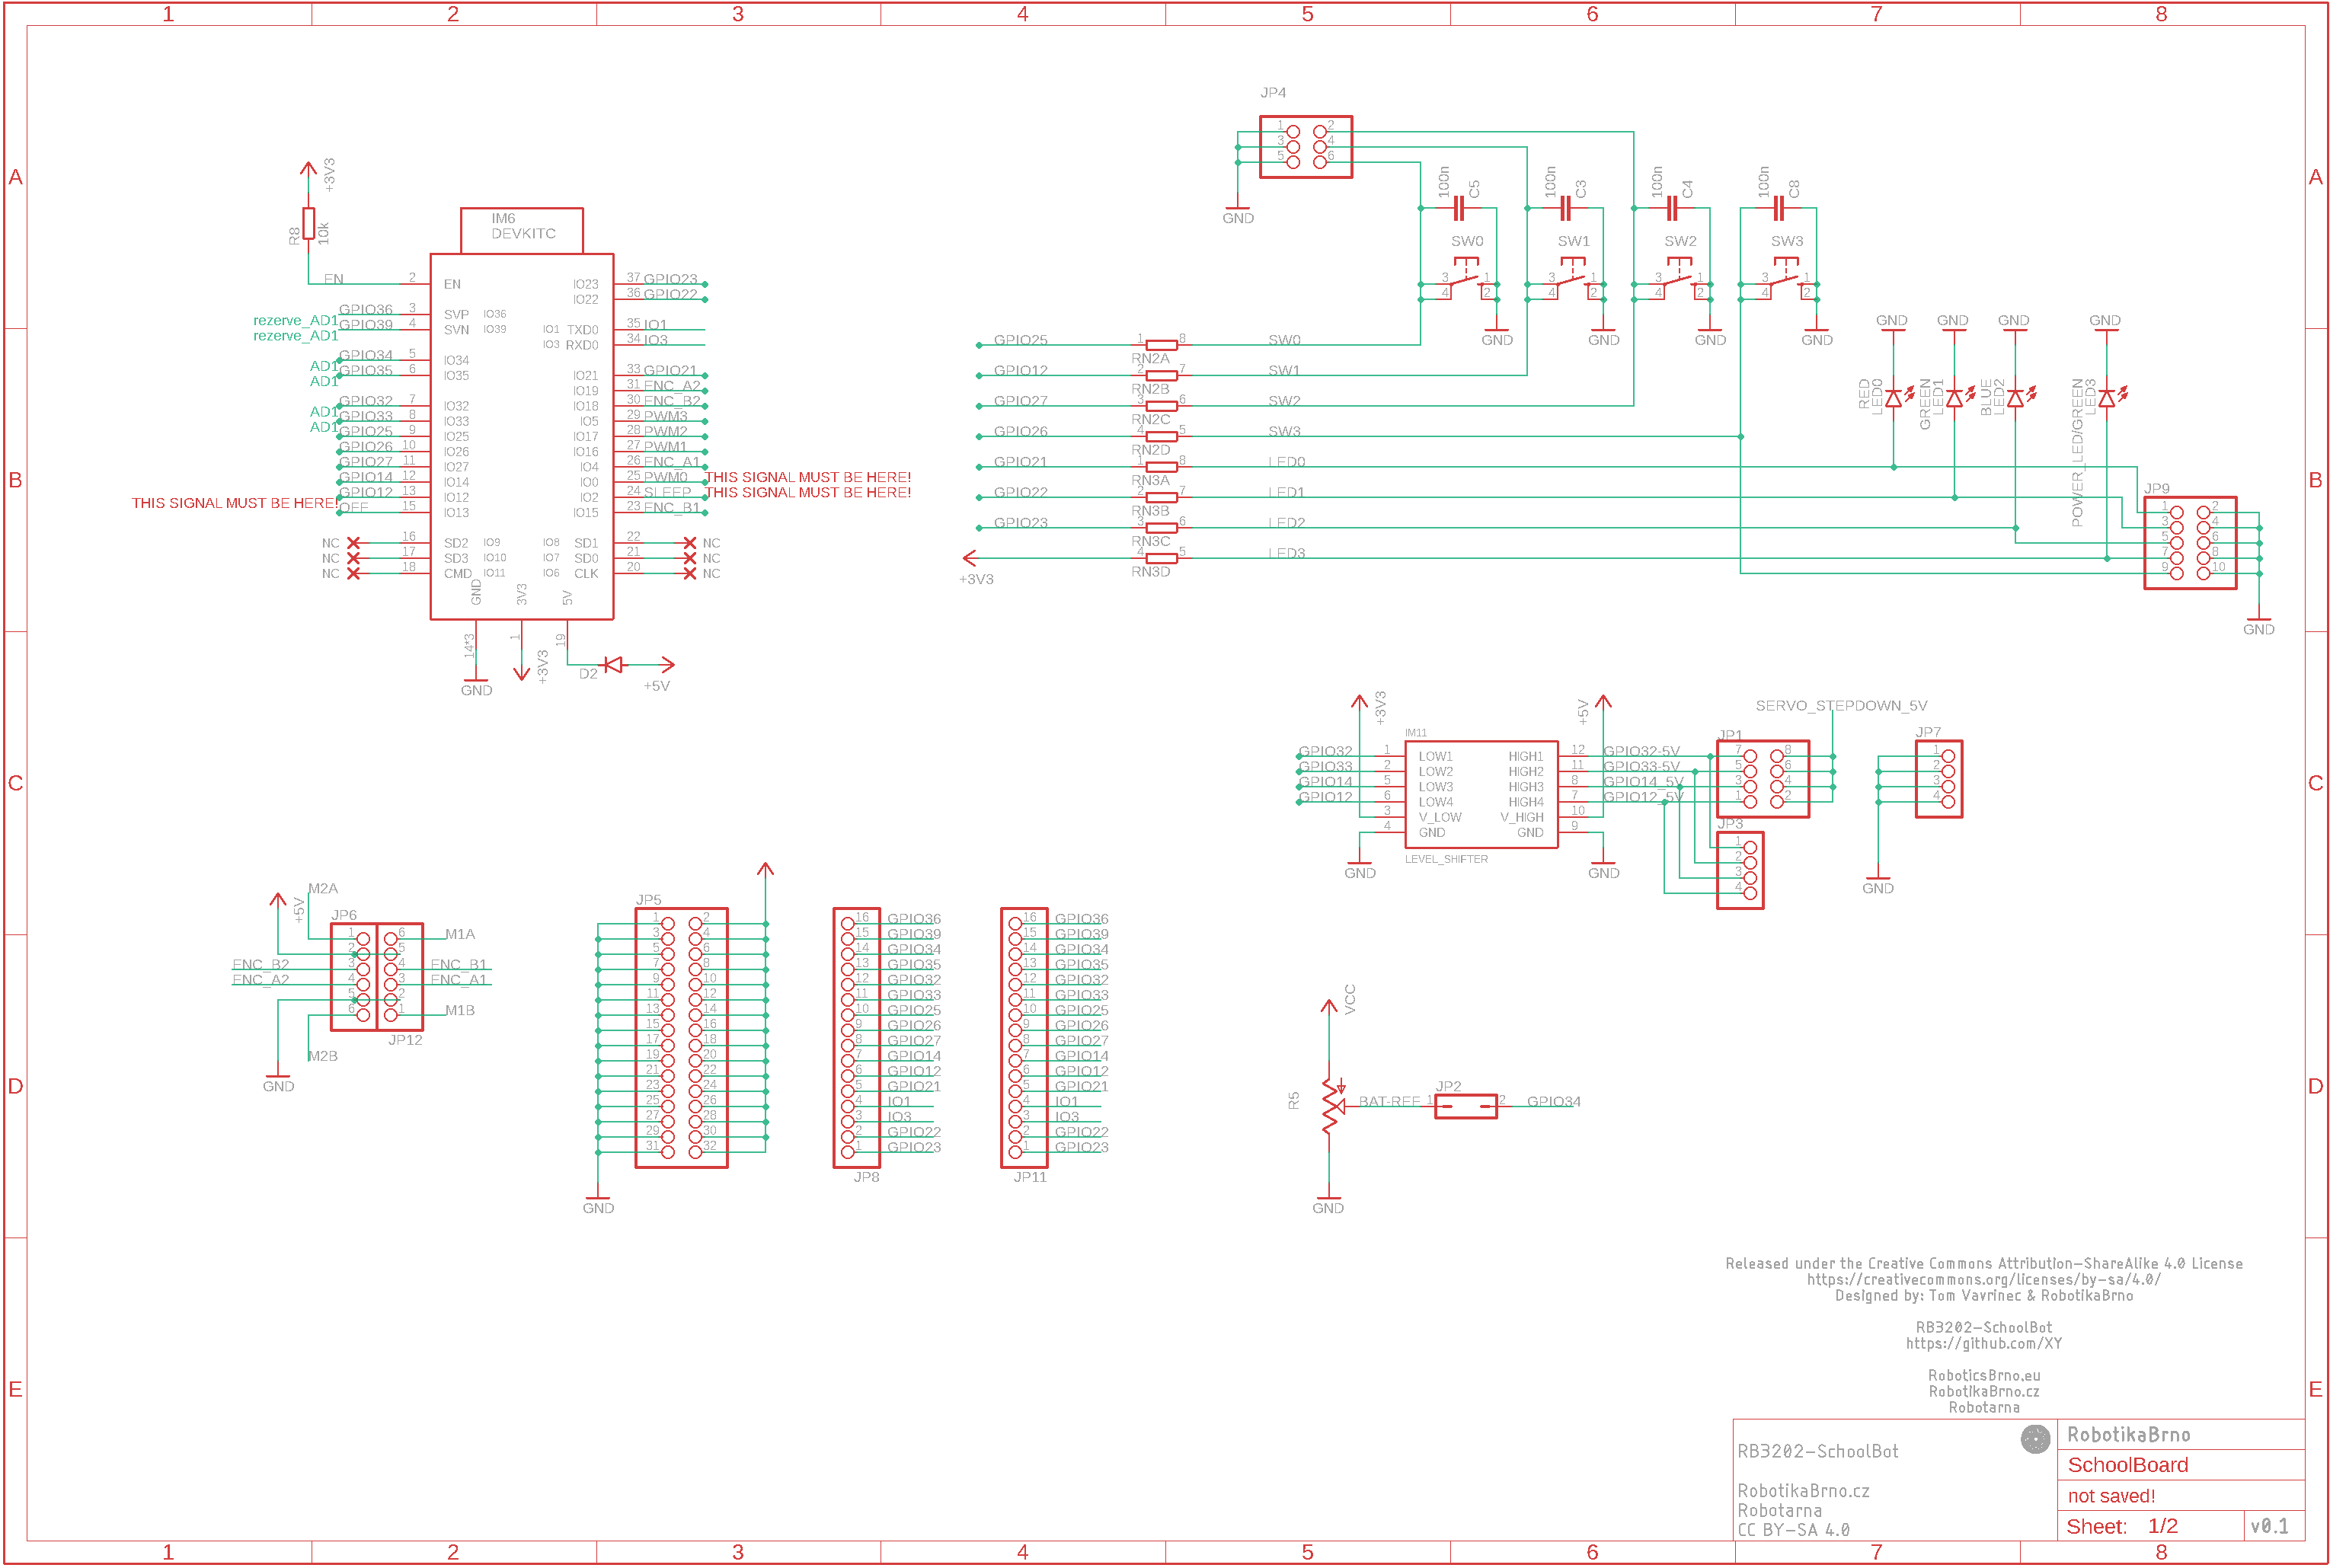
\includegraphics[width=1.5\textwidth, angle = 90]{img/logika.png}
	\caption{schéma logické části desky}
\end{figure}

\begin{figure}[h]
	\centering
	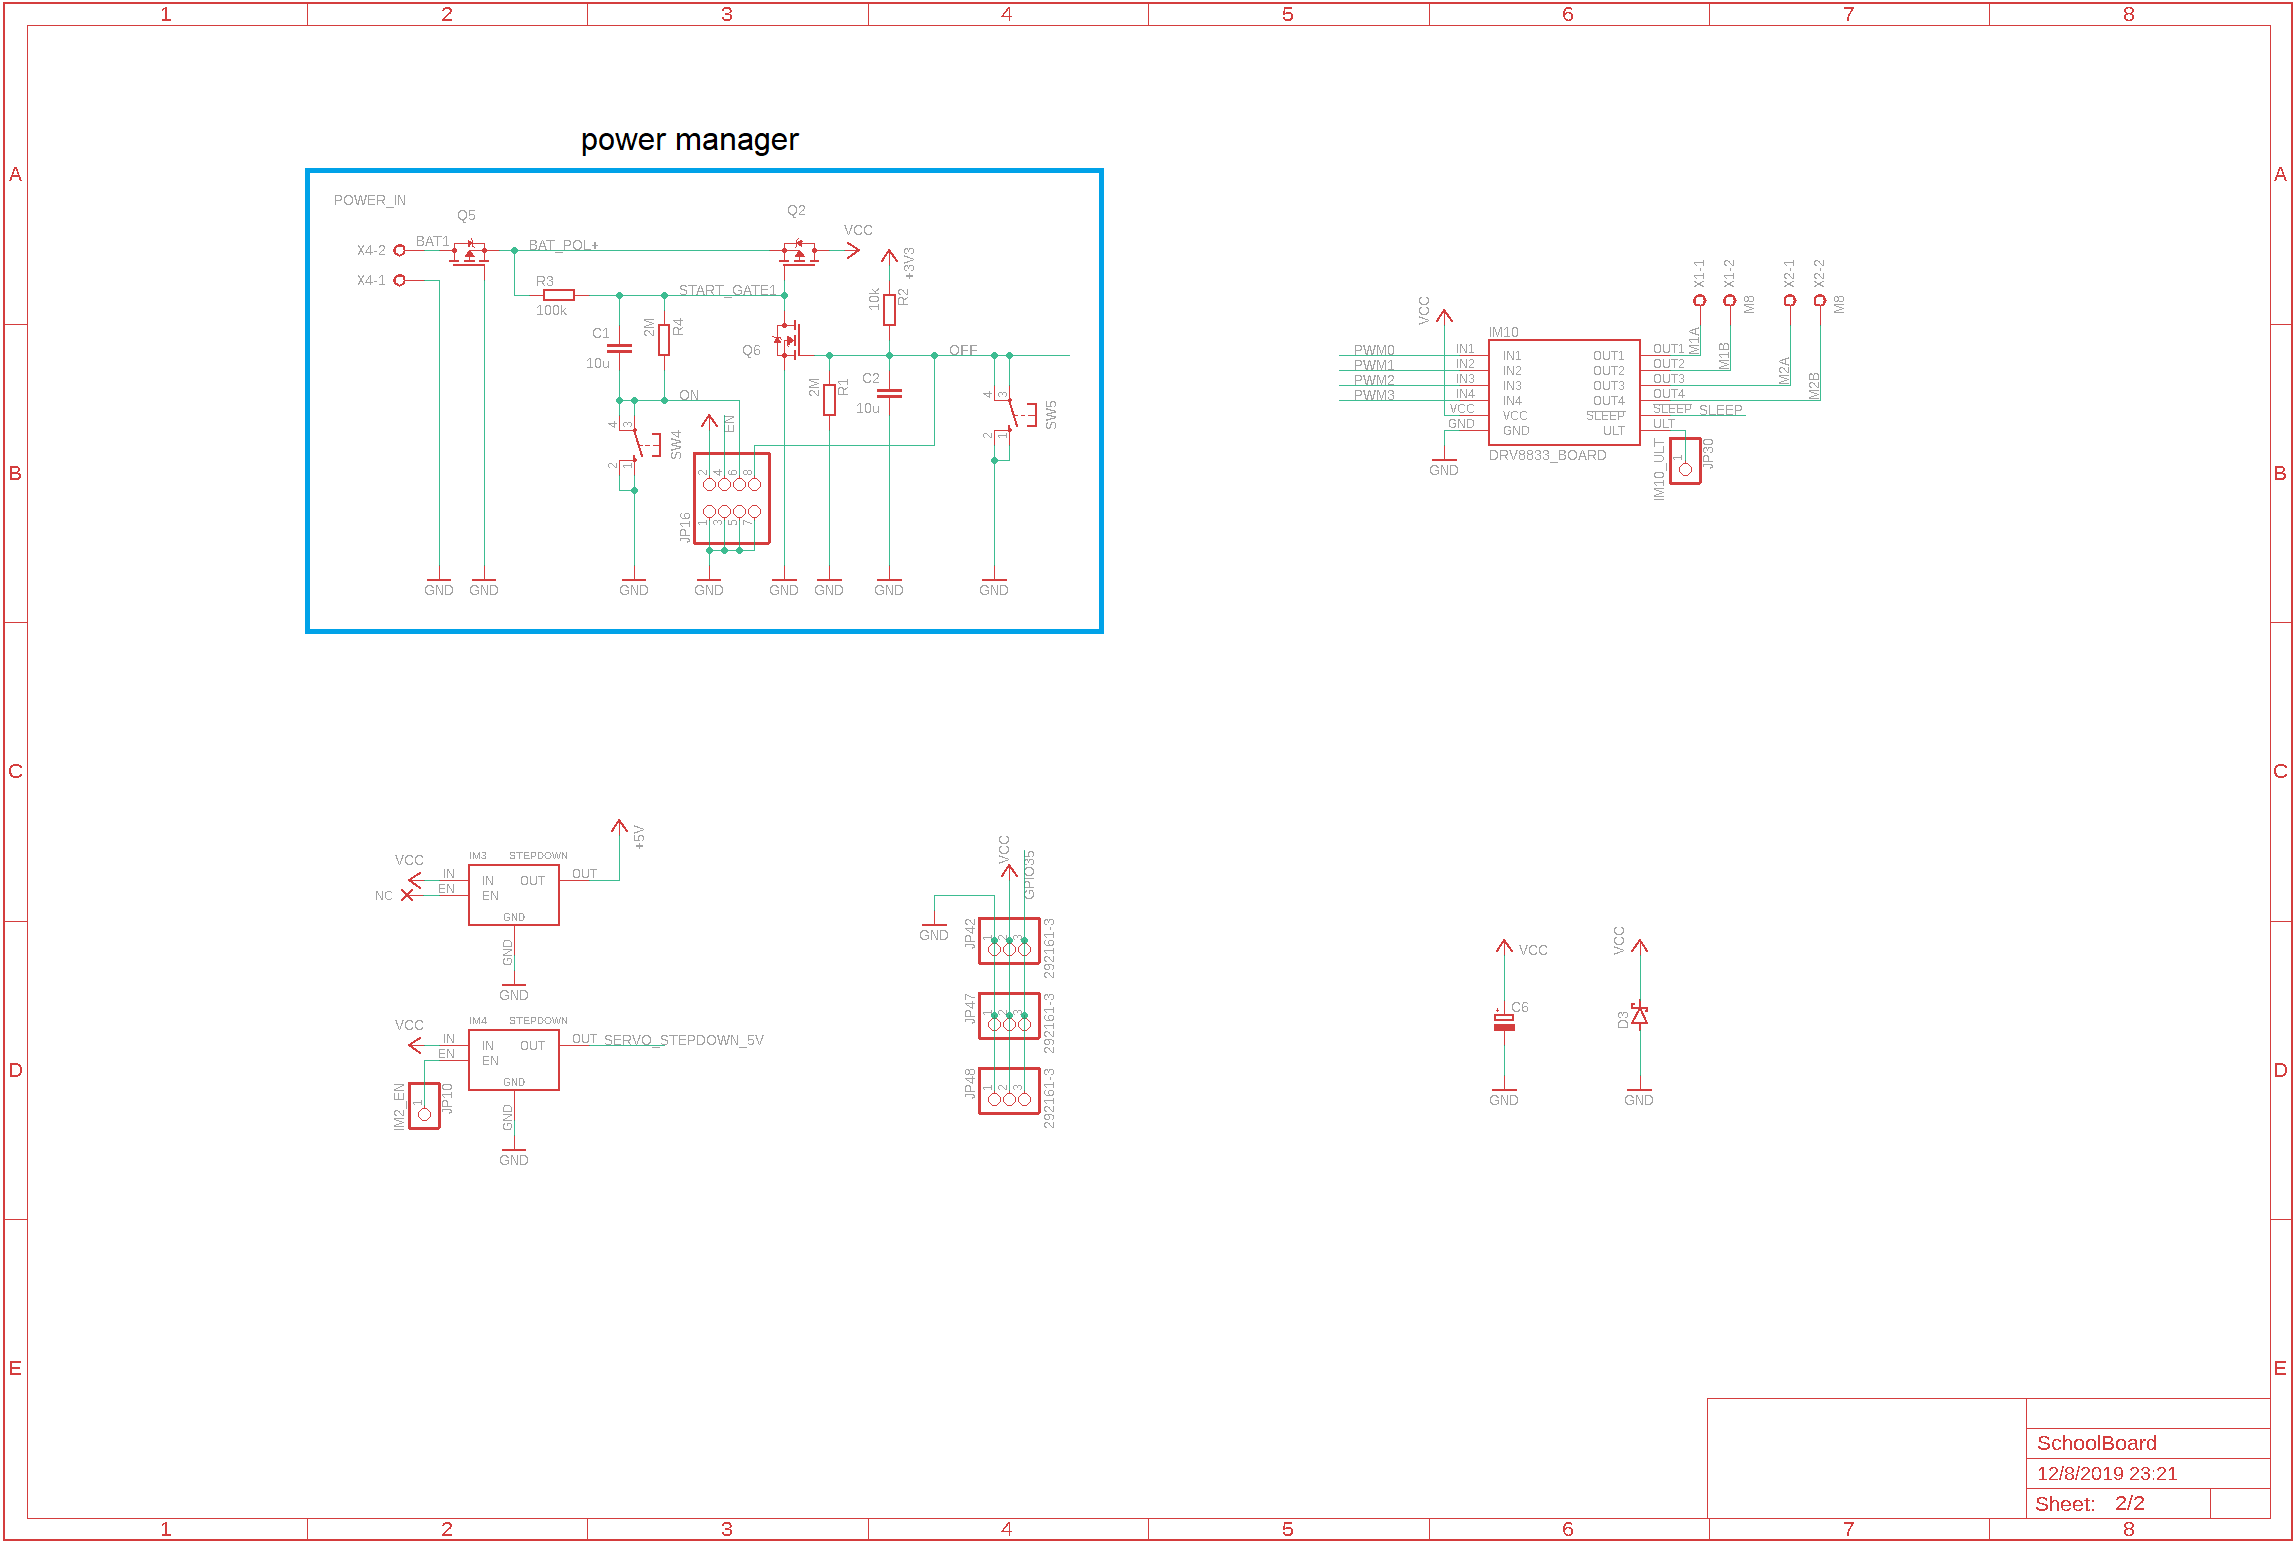
\includegraphics[width=1.5\textwidth, angle = 90]{img/silovka.png}
	\caption{schéma výkonové části}
\end{figure}

%%%%%%%%%%%%%%%%%%%%%%%%%%%%%%%%%%%%%%%%%%%%%%%%%%%%
\newpage
\printbibliography[title=Literatura]

\addcontentsline{toc}{section}{Literatura}

\listoffigures
\addcontentsline{toc}{section}{Seznam obrázků}

\listoftables
\addcontentsline{toc}{section}{Seznam tabulek}
\renewcommand{\refname}{Další zdroje}
\begin{thebibliography}{1}
	
	\subsection*{LEGO Mindstorm}
	
	\bibitem{LEGO Mindstorm} 
	\textit{porovnání cen LEGa} [online] www.heureka.cz [cit. 2020-02-22] Dostupné z: \\ 
	\url{https://lego.heureka.cz/lego-mindstorms-31313-ev3/#o=2}
	
	
	\subsection*{Mbot}
	\bibitem{Mbot} 
	\textit{Mbot} [online] https://www.makeblock.com/mbot [cit. 2020-02-22] Dostupné z: \url{https://www.makeblock.com/mbot}
	
	
	\subsection*{Edison V2.0}
	\bibitem{Edison V2.0} 
	\textit{Meet Edison. Wiltronics | Science and Technology product specialists} [online] [cit. 2020-02-22] Dostupné z: \url{https://www.wiltronics.com.au/MeetEdison/}
	
	\bibitem{Edison V2.0}
	\textit{Introducing Edison V2.0 - the newest version of the Edison robot. Edison Programmable Robot - Ideal for school classroom education} [online] [cit. 2020-02-22] Dostupné z:
	\url{https://meetedison.com/meet-edison-v2-0/}
	
	\bibitem{Edison V2.0}
	\textit{příklad ceny} [online] [cit. 2020-02-22] Dostupné z: \\ 
	\url{https://www.robotshop.com/ca/en/edison-programmable-v20-robot.html?gclid=Cj0KCQiA4sjyBRC5ARIsAEHsELHtKqVNJOl95kMUC8iBngIkgc3gCZU9KOTwuXWEo4hU4Qs1B-2wASkaAh9CEALw_wcB}
	
	\subsection*{OZOBOT}
	
	\bibitem{OZOBOT} 
	\textit{OZOBOT} [online] [cit. 2020-02-22] Dostupné z:
	\url{https://www.youtube.com/watch?v=lqR3zDWAQ1o}
	
	\bibitem{OZOBOT}
	\textit{OZOBOT} [online] [cit. 2020-02-22] Dostupné z:
	\url{https://www.youtube.com/watch?v=Cw30OdlczRo}
	
	\subsection*{Asuro}
	
	\bibitem{Asuro} 
	\textit{Asuro} [online] [cit. 2020-02-22] Dostupné z:
	\url{ http://www.arexx.com/downloads/asuro/asuro_manual_en.pdf}
	
	\bibitem{Asuro}
	\textit{Programovatelný robot ASURO ARX-3 USB - Vyhledávání na Heureka.cz. Heureka.cz - Porovnání cen a srovnání produktů z internetových obchodů } [online] [cit. 2020-02-22] Dostupné z:
	\url{https://www.heureka.cz/?h[fraze]=Programovateln%C3%BD+robot+ASURO+ARX-3+USB}
		
		\bibitem{Asuro}
		\textit{2012 Kurz zakladni robotiky - robot ASURO - talentovaní.cz. Talentovaní.cz - talentovaní.cz} [online] [cit. 2020-02-22] Dostupné z:
		\url{https://vtp.talentovani.cz//2012 kurz-zakladni-robotiky-robot-asuro}
		
		\subsection*{Microbit}
		
		\bibitem{Microbit} 
		\textit{Micro:bit Educational Foundation | micro:bit. Micro:bit Educational Foundation | micro:bit} [online] [cit. 2020-02-22] Dostupné z:
		\url{https://microbit.org/}
		
		\bibitem{Microbit}
		\textit{Cutebot - Micro:bit chytré auto - HW Kitchen. Ochutnejte s námi bastlení! | HWKitchen.cz} [online] [cit. 2020-02-22] Dostupné z:
		\url{https://www.heureka.cz/?h[fraze]=Programovateln%C3%BD+robot+ASURO+ARX-3+USB}
			
			%\subsection*{použité součástky}
			
			\subsection*{součásti desky SchoolBoard}
			
			%\paragraph*{ESP32}
			
			\bibitem{WROOM}
			\textit{Espressif Systems - Wi-Fi and Bluetooth chipsets and solutions } [online] [cit. 2020-02-22] Dostupné z:
			\url{https://www.espressif.com/sites/default/files/documentation/esp32-wroom-32_datasheet_en.pdf}
			
			\bibitem{ESP32}
			\textit{datasheet ESP32} [online] [cit. 2020-02-22] Dostupné z:
			\url{https://cdn.sparkfun.com/datasheets/IoT/esp32_datasheet_en.pdf}
			
			\bibitem{ESP32_II} %todo proč dva datasheety? 
			\textit{datasheet ESP32} [online] [cit. 2020-02-22] Dostupné z:
			\url{https://pdf1.alldatasheet.com/datasheet-pdf/view/1148023/ESPRESSIF/ESP32.html}
			
			%\paragraph*{DRV8833 (motorový driver)}
			
			\bibitem{DRV8833}
			\textit{datasheet DRV8833} [online] [cit. 2020-02-22] Dostupné z:
			\url{http://www.ti.com/lit/ds/symlink/drv8833.pdf}
			
			%\paragraph*{IRF4905}
			
			\bibitem{IRF4905}
			\textit{datasheet IRF4905} [online] [cit. 2020-02-22] Dostupné z:
			\url{https://www.infineon.com/dgdl/irf4905pbf.pdf?fileId=5546d462533600a4015355e329b1197e}
			
			%\paragraph*{BS170}
			
			\bibitem{BS170}
			\textit{datasheet BS170} [online] [cit. 2020-02-22] Dostupné z:
			\url{https://www.onsemi.com/pub/Collateral/BS170-D.PDF}
			
			%\paragraph*{7805}
			
			\bibitem{7805}
			\textit{datasheet 7805} [online] [cit. 2020-02-22] Dostupné z:
			\url{https://www.st.com/resource/en/datasheet/l78.pdf}
			
			%\paragraph*{Step-down}
			
			\bibitem{Step-down}
			\textit{datasheet Step-down} [online] [cit. 2020-02-22] Dostupné z:
			\url{https://arduino-shop.cz/docs/produkty/0/698/1502185417.pdf}
			
			%\paragraph*{Mikrospínač}
			
			\bibitem{mikrospinac}
			\textit{datasheet -- mikrospínač} [online] [cit. 2020-02-22] Dostupné z:
			\url{https://www.gme.cz/data/attachments/dsh.630-019.1.pdf}
			
			\subsection*{inteligentní servo LX15D}
			
			\bibitem{inteligentni_serva_LX15D}
			\textit{inteligentní serva LX15D} [online] [cit. 2020-02-22] Dostupné z:
			\url{http://www.lewansoul.com/product/detail-7.html}
			
		\end{thebibliography}

\end{document}


